\documentclass[12pt]{amsart}
\usepackage{amsmath}
\usepackage{tikz,float,caption}
\usetikzlibrary{arrows.meta,calc,decorations.markings,patterns,cd,patterns.meta}

\begin{document}

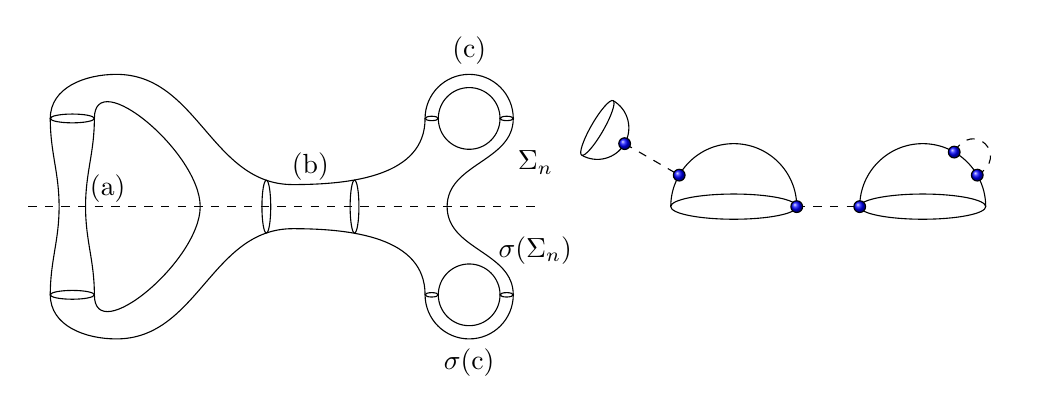
\begin{tikzpicture}[scale=.8]
    \begin{scope}[scale=0.7]
      \node at (.8,.4) {(a)};
      \node at (5.4,.9) {(b)};
      \node at (9.0,3)[above] {(c)};
      \node at (10.5,1) {$\Sigma_{n}$};
      \draw (-0.3,0) to[out=90,in=-90] (-.5,2) to[out=90,in=180] (1,3) to[out=0,in=180] (5,.5) to [out=0,in=-90] (8,2) arc (180:0:1) to[out=270,in=90] (8.5,0);
      \draw (0.3,0) to[out=90,in=-90] (0.5,2) to[out=90,in=90] (2.9,0);
      \draw (0,2) circle (0.5 and 0.1);
      \draw (9,2) circle (0.7 and 0.7);
      \draw (4.4,0) circle (0.1 and .6);
      \draw (6.4,0) circle (0.1 and .6);
      \draw (8.15,2) circle (0.15 and 0.05);
      \draw (10-.15,2) circle (0.15 and 0.05);
      \draw[dashed] (-1,0)--(10.5,0);
      \begin{scope}[yscale=-1]
        \node at (10.5,1) {$\sigma(\Sigma_{n})$};
        \draw (-0.3,0) to[out=90,in=-90] (-.5,2) to[out=90,in=180] (1,3) to[out=0,in=180] (5,.5) to [out=0,in=-90] (8,2) arc (180:0:1) to[out=270,in=90] (8.5,0);
        \draw (0.3,0) to[out=90,in=-90] (0.5,2) to[out=90,in=90] (2.9,0);
        \draw (0,2) circle (0.5 and 0.1);
        \draw (9,2) circle (0.7 and 0.7);
        \draw (8.15,2) circle (0.15 and 0.05);
        \draw (10-.15,2) circle (0.15 and 0.05);
        \node at (9.0,3)[below] {$\sigma(\mathrm{c})$};
      \end{scope}
    \end{scope}   
    \begin{scope}[shift={(10.5,0)},every node/.style={draw,circle,shading=ball,inner sep=1.5pt}]

      \draw [dashed] (1,0)--(2,0);
      \draw (1,0) arc (0:180:1) (0,0) circle (1 and 0.2) (3,0) circle (1 and 0.2) (4,0) arc (0:180:1);
      \begin{scope}[shift={(150:2.5)},rotate=-120]
        \draw (0.5,0) arc (0:180:.5);
        \draw (0,0) circle (0.5 and 0.1);
        \draw[dashed] (0,.5)--(0,1.5);
        \node at (0,.5) {};
        \node at (0,1.5) {};
      \end{scope}

      \begin{scope}[shift={(3,0)}]
        \draw[dashed] (30:1) to[out=30,in={60},looseness=3] (60:1);
        \node at (-1,0) {};
        \node at (30:1) {};
        \node at (60:1) {};
      \end{scope}
      \node at (1,0) {};
    \end{scope}
  \end{tikzpicture}

\end{document}